\section{Visual Identity, 3D Model and UX}
\label{sec:visual-identity-ux}

The visual language of AHI is a dark mission control look: deep navy backgrounds, translucent glass panels, a teal accent and five status colors that always come with words and an icon. This section defines the design system of the platform, the frontend technologies that implement it and the 3D anatomical model at the center of the interface. The interface is in English, because the work is presented to an international audience, and it states plain language first and the technical term second.

Three principles guided the design. \textbf{Plain language first}, so that a person under stress reads "Act soon" before "Warning". \textbf{Honesty about data}, so that the origin of the data and the loss of a signal are always visible. And \textbf{one source of truth with two views}, so that the astronaut and the flight surgeon see the same state in layouts made for their needs.

\subsection{Frontend Technologies}
\label{subsec:frontend-technologies}

The interface is a single page web application written in TypeScript. \ref{tab:frontend-stack} lists the main tools and the role of each one. The versions are those declared in the project at the time of writing.

\begin{table}[htbp]
\centering
\vspace{0.8em}
\caption{Main frontend technologies of AHI.}
\label{tab:frontend-stack}
\footnotesize
\begin{tabular}{p{3.6cm}p{1.6cm}p{8.8cm}}
\hline
\textbf{Tool} & \textbf{Version} & \textbf{Role} \\
\hline
React & 19 & Component model of the whole interface \\
TypeScript & 7 & Typed code and the shared data contract between the engine and the interface \\
Vite & 8 & Development server and production build, with code splitting so the 3D viewer loads on demand \\
Tailwind CSS & 4 & Design tokens and styling of every screen \\
zustand & 5 & Application state store that owns the analytical engine and publishes only the parts of the state that changed \\
Recharts & 3 & Trend charts with the personal band, gaps for missing data and forecast cones \\
lucide-react & 1 & Icon set used with every status word \\
three.js & 0.187 & WebGL rendering of the 3D body \\
React Three Fiber & 9 & React renderer for three.js, so the 3D scene follows the same component model \\
drei & 10 & three.js helpers: orbit controls, procedural lighting environment, contact shadows, bounding volume hierarchies for picking \\
postprocessing & 6 & Bloom on status highlights and filmic tone mapping \\
glTF Transform and meshoptimizer & 4.5 and 1.3 & Build time optimization and compression of the 3D model files \\
Blender & 4.5 LTS & Headless preparation of the anatomical source model at build time \\
Vitest and oxlint & 5 and 1 & Unit tests and static checks \\
\hline
\end{tabular}
\vspace{1.2em}
\end{table}

The analytical engine is written in the same language and runs in the same application, so the interface reads its results directly from the store. Charts and the 3D scene read live values without forcing the rest of the interface to render again, which keeps the screen responsive while the data update every simulated minute.

% AHI design tokens (frontend/web/src/index.css and src/lib/status.ts)
\definecolor{ahiSpace950}{HTML}{04070D}
\definecolor{ahiSpace900}{HTML}{070C16}
\definecolor{ahiSpace850}{HTML}{0A1120}
\definecolor{ahiSpace800}{HTML}{0E1729}
\definecolor{ahiSpace700}{HTML}{16223A}
\definecolor{ahiSpace600}{HTML}{22324F}
\definecolor{ahiInk100}{HTML}{E8EEFC}
\definecolor{ahiInk300}{HTML}{A9B6CF}
\definecolor{ahiInk500}{HTML}{7D8BA6}
\definecolor{ahiAccent}{HTML}{5EEAD4}
\definecolor{ahiAccentStrong}{HTML}{2DD4BF}
\definecolor{ahiSky}{HTML}{7DD3FC}
\definecolor{ahiNominal}{HTML}{34D399}
\definecolor{ahiWatch}{HTML}{FBBF24}
\definecolor{ahiWarning}{HTML}{FB923C}
\definecolor{ahiCritical}{HTML}{F43F5E}
\definecolor{ahiNoData}{HTML}{94A3B8}
\definecolor{ahiViolet}{HTML}{A78BFA}
\definecolor{ahiVioletText}{HTML}{DDD6FE}
\newcommand{\swatch}[1]{{\setlength{\fboxsep}{0pt}\setlength{\fboxrule}{0.3pt}\fcolorbox{black!35}{#1}{\rule{0pt}{0.85em}\rule{2.2em}{0pt}}}}
\newcommand{\statuspill}[2]{\tikz[baseline=-0.6ex]\node[fill=#1,rounded corners=5pt,inner xsep=7pt,inner ysep=3.5pt,text=ahiSpace900,font=\footnotesize\bfseries]{#2};}

\subsection{Logo}
\label{subsec:logo}

The logo of AHI, shown in \ref{fig:ahi-logo}, is a mark drawn in vector form and a wordmark. The mark combines a circle, a tilted orbit, a small point on that orbit and a heartbeat trace across the center: a body in orbit and its vital signs, which is what the platform watches. Its strokes use a gradient from the teal accent to a light sky blue, and it sits on the deep navy background of the interface. In the application the mark appears in the top bar next to the wordmark ``AHI'', and the documentation portal uses the same mark.

\hwfigure{0.80}{images/branding/ahi-logo.png}{AHI logo: the mark (circle, orbit, orbiting point and heartbeat trace) with the wordmark on the interface background. The full name below the wordmark was added for this report.}{fig:ahi-logo}{Rendered by the authors from the AHI logo source (\texttt{frontend/web/src/features/topbar/TopBar.tsx} and \texttt{docs-site/public/logo.svg}).}

\subsection{Color Palette}
\label{subsec:color-palette}

Status is the only use of the five signal colors, never decoration. \ref{tab:status-language} defines the status language, which is declared once and used by every screen and by the 3D body. Color is never the only cue: every status pairs its color with an icon and a word, and the missing data status changes shape as well.

\begin{table}[htbp]
\centering
\vspace{0.8em}
\caption{Status language: wording, technical label, color and shape.}
\label{tab:status-language}
\small
\begin{tabular}{p{2.2cm}p{2.4cm}p{2.4cm}p{2.8cm}p{3.8cm}}
\hline
\textbf{Status} & \textbf{Crew wording} & \textbf{Technical label} & \textbf{Color} & \textbf{Dot and animation} \\
\hline
Low & All good & Nominal & \swatch{ahiNominal}\ \texttt{\#34D399} & Filled \\
Moderate & Keep an eye & Watch & \swatch{ahiWatch}\ \texttt{\#FBBF24} & Filled \\
High & Act soon & Warning & \swatch{ahiWarning}\ \texttt{\#FB923C} & Filled, slow pulse \\
Critical & Act now & Critical & \swatch{ahiCritical}\ \texttt{\#F43F5E} & Filled, fast pulse \\
No data & Signal lost & No data & \swatch{ahiNoData}\ \texttt{\#94A3B8} & Hollow and dashed, never filled \\
\hline
\end{tabular}
\vspace{1.2em}
\end{table}

The no data status is deliberately different from the low status, so that \textbf{missing data never reads as normal}. In the 3D body the nominal regions use calm, cool tints, so that any warm color reads as attention, and a region with no data is grey, dimmed and still.

Backgrounds use a scale of deep navy tones from near black to a lighter slate. Text uses three levels of light grey for primary, secondary and muted content. A teal accent marks focus rings, links and the spotlight of the guided demonstration. Data origin badges follow a consistent scheme, and whenever simulated data are shown, for development, training or demonstration, a violet badge marked simulated is always visible in the top bar.

\ref{fig:status-preview} shows the five status colors as they appear on the interface background, and \ref{tab:palette} lists the full palette, with the token name used in the code, the color and its use.

\par\bigskip\noindent
\begin{minipage}{\linewidth}
\centering
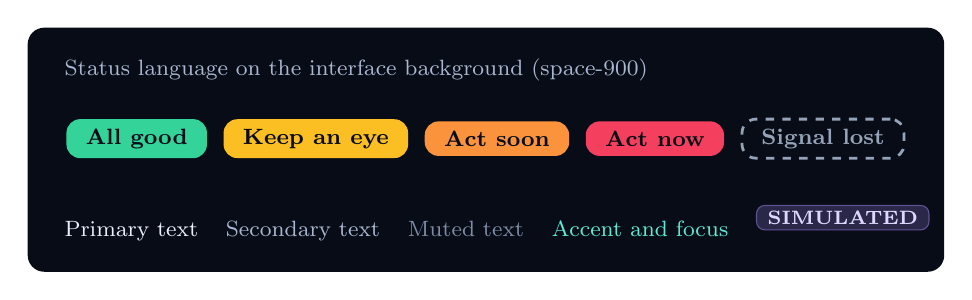
\begin{tikzpicture}
\node[fill=ahiSpace900,rounded corners=6pt,minimum width=0.96\linewidth,minimum height=3.1cm] (bg) {};
\node[anchor=north west,text=ahiInk300,font=\footnotesize] at ([xshift=10pt,yshift=-8pt]bg.north west) {Status language on the interface background (space-900)};
\node at ([yshift=4pt]bg.center) {\statuspill{ahiNominal}{All good}\hspace{6pt}\statuspill{ahiWatch}{Keep an eye}\hspace{6pt}\statuspill{ahiWarning}{Act soon}\hspace{6pt}\statuspill{ahiCritical}{Act now}\hspace{6pt}\tikz[baseline=-0.6ex]\node[draw=ahiNoData,dashed,line width=1pt,rounded corners=5pt,inner xsep=7pt,inner ysep=3.5pt,text=ahiNoData,font=\footnotesize\bfseries]{Signal lost};};
\node[anchor=south west,font=\footnotesize] at ([xshift=10pt,yshift=8pt]bg.south west) {\textcolor{ahiInk100}{Primary text}\hspace{10pt}\textcolor{ahiInk300}{Secondary text}\hspace{10pt}\textcolor{ahiInk500}{Muted text}\hspace{10pt}\textcolor{ahiAccent}{Accent and focus}\hspace{10pt}\tikz[baseline=-0.6ex]\node[fill=ahiViolet!22!ahiSpace900,draw=ahiViolet!55!ahiSpace900,rounded corners=3pt,inner xsep=4pt,inner ysep=2pt,text=ahiVioletText,font=\scriptsize\bfseries]{SIMULATED};};
\end{tikzpicture}
\captionof{figure}{Status pills, text levels, accent and the simulated data badge drawn with the real colors of the interface.}
\label{fig:status-preview}
\figsource{Drawn by the authors from the AHI design tokens (\texttt{frontend/web/src/index.css} and \texttt{frontend/web/src/lib/status.ts}).}
\end{minipage}
\par\bigskip

\begin{table}[htbp]
\centering
\vspace{0.8em}
\caption{AHI color palette, from the design tokens of the interface.}
\label{tab:palette}
\footnotesize
\begin{tabular}{p{2.6cm}p{2.9cm}p{8.5cm}}
\hline
\textbf{Token} & \textbf{Color} & \textbf{Use} \\
\hline
\multicolumn{3}{l}{\textit{Backgrounds}} \\
\texttt{space-950} & \swatch{ahiSpace950}\ \texttt{\#04070D} & Deepest background, behind the 3D scene \\
\texttt{space-900} & \swatch{ahiSpace900}\ \texttt{\#070C16} & Main page background \\
\texttt{space-850} & \swatch{ahiSpace850}\ \texttt{\#0A1120} & Panels \\
\texttt{space-800} & \swatch{ahiSpace800}\ \texttt{\#0E1729} & Raised panels and cards \\
\texttt{space-700} & \swatch{ahiSpace700}\ \texttt{\#16223A} & Borders and hover surfaces \\
\texttt{space-600} & \swatch{ahiSpace600}\ \texttt{\#22324F} & Dividers and inactive controls \\
\multicolumn{3}{l}{\textit{Text}} \\
\texttt{ink-100} & \swatch{ahiInk100}\ \texttt{\#E8EEFC} & Primary text and values \\
\texttt{ink-300} & \swatch{ahiInk300}\ \texttt{\#A9B6CF} & Secondary text \\
\texttt{ink-500} & \swatch{ahiInk500}\ \texttt{\#7D8BA6} & Muted text, axis labels \\
\multicolumn{3}{l}{\textit{Brand and accent}} \\
\texttt{accent} & \swatch{ahiAccent}\ \texttt{\#5EEAD4} & Focus rings, links, demonstration spotlight, start of the logo gradient \\
\texttt{accent-strong} & \swatch{ahiAccentStrong}\ \texttt{\#2DD4BF} & Pressed and active states \\
Logo gradient end & \swatch{ahiSky}\ \texttt{\#7DD3FC} & End of the logo gradient \\
\multicolumn{3}{l}{\textit{Status (only for status, never decoration)}} \\
\texttt{nominal} & \swatch{ahiNominal}\ \texttt{\#34D399} & Low: all good \\
\texttt{watch} & \swatch{ahiWatch}\ \texttt{\#FBBF24} & Moderate: keep an eye \\
\texttt{warning} & \swatch{ahiWarning}\ \texttt{\#FB923C} & High: act soon \\
\texttt{critical} & \swatch{ahiCritical}\ \texttt{\#F43F5E} & Critical: act now \\
\texttt{nodata} & \swatch{ahiNoData}\ \texttt{\#94A3B8} & No data: signal lost \\
\multicolumn{3}{l}{\textit{Data origin}} \\
Simulated badge & \swatch{ahiViolet}\ \texttt{\#A78BFA} & Violet badge for simulated data (Tailwind violet; text in \texttt{\#DDD6FE}) \\
\hline
\end{tabular}
\vspace{1.2em}
\end{table}


\subsection{Typography}
\label{subsec:typography}

The interface uses the Inter family for text and JetBrains Mono for numbers and codes. Numbers use tabular figures, so that live values do not jitter as digits change. In presentation mode no text is smaller than 13 pixels, chart ticks included. The fonts are bundled with the application, so that the on board interface makes no external request.

\subsection{Components}
\label{subsec:ui-components}

The interface is assembled from a small set of shared components:

\begin{itemize}
\item \textbf{Status pill, icon and dot:} the status language of \ref{tab:status-language}.
\item \textbf{Metric value:} numbers that change smoothly, and that snap when reduced motion is requested or the page is hidden.
\item \textbf{Trend chart:} the personal band labeled "Your normal", gaps wherever data is missing, the forecast cone and markers for alerts, actions and check-ins. Gaps stay gaps: missing data is never filled or smoothed over.
\item \textbf{Sparkline:} six hours of history in crew cards and in the vitals strip.
\item \textbf{Risk gauge:} the score from 0 to 100 with its level.
\item \textbf{Baseline explanation:} a "Why is this my normal?" control that shows the window, the readings, the median and the MAD.
\item \textbf{Autonomy badge:} "Can act on board now", "Needs flight surgeon" or the minimum wait for an Earth reply.
\item \textbf{Origin badge:} the data origin of every value.
\end{itemize}

Several decisions follow from these components. The Crew view shows at most two actions, to reduce the load, and the rest is available in the Ground view. Every recommendation says who can act, because communication delay makes autonomy part of the answer. The critical banner floats over the header of the central area, so that the 3D body keeps its size during an alert.

Accessibility is part of the design: global keyboard shortcuts, keyboard navigation of timeline markers, a visible focus ring, a link that skips to what needs attention as the first focusable element, and accessible labels on every control. The target is conformance with WCAG 2.1 level AA, verified by a formal audit and by tests with a screen reader. The ground screens are designed for large displays, and the Crew view also for the tablets and laptops used on board.

\subsection{3D Anatomical Model}
\label{subsec:3d-model}

The body in the center of the interface is a \textbf{real anatomical atlas}: the open Z-Anatomy model, ``the libre 3D atlas of anatomy'', itself based on BodyParts3D \cite{z_anatomy}. It was chosen because it covers the whole body with named structures organized by anatomical system, which is what layers, selection and the link to health data need, and because its Blender source can be processed automatically and reproducibly. Z-Anatomy is distributed under the Creative Commons Attribution-ShareAlike 4.0 license, so the derived files are shared under the same license with its attribution, shown in a caption under the body that is always visible. The atlas is one adult reference body shown for every crew member. It is not a scan of an astronaut, and its colors come from the health data, never from the model.

\medskip\noindent\textbf{Asset pipeline.} The published files are generated by scripts and never edited by hand. One command runs the whole chain in about five minutes:

\begin{enumerate}
\item \textbf{Source.} The Z-Anatomy archive is downloaded from one allowed host and checked against a pinned SHA-256 hash.
\item \textbf{Blender export.} Blender 4.5 LTS runs headless, with embedded scripts disabled. It keeps only physical bodies, converts vessel and nerve curves into tubes, joins about 2,230 source objects into 250 structures, removes about four fifths of the triangles, moves the body to the viewer frame and writes one file per anatomical system.
\item \textbf{Kidneys.} The upstream kidney model has a non commercial license, so AHI builds its own kidneys in code and fits them to the size and position of the atlas kidneys.
\item \textbf{Optimization.} glTF Transform and meshoptimizer remove duplicates, quantize positions and normals and compress every file.
\item \textbf{Validation.} The published files are checked against a manifest contract that lists every structure with its system, tissue, side, bounding box and origin. Automated tests fail if a required structure is missing or an excluded object appears.
\end{enumerate}

Some upstream content was left out on purpose: the inner ear and the kidney, because of non commercial licenses, reproductive structures, so that the model is a neutral reference body, and helper objects such as labels. \ref{tab:3d-systems} summarizes the result.

\begin{table}[htbp]
\centering
\vspace{0.8em}
\caption{Files of the 3D anatomical model, one per anatomical system.}
\label{tab:3d-systems}
\footnotesize
\begin{tabular}{p{2.6cm}p{6.6cm}p{1.6cm}p{1.6cm}p{1.2cm}}
\hline
\textbf{System} & \textbf{Content} & \textbf{Structures} & \textbf{Triangles} & \textbf{MB} \\
\hline
Integumentary & Skin, the whole body surface & 1 & 48,503 & 0.24 \\
Skeletal & Skull, vertebrae, ribs, sternum and limb bones & 41 & 184,971 & 0.95 \\
Muscular & Large muscles one by one, small ones by group & 133 & 299,818 & 1.66 \\
Cardiovascular & Heart, coronary vessels, great vessels, arteries and veins & 29 & 89,893 & 0.50 \\
Respiratory & Lungs, trachea, bronchi, larynx, diaphragm & 6 & 44,991 & 0.22 \\
Nervous & Brain, cerebellum, brainstem, spinal cord, nerves & 17 & 133,356 & 0.66 \\
Digestive & Tongue to intestines, liver, gallbladder, pancreas & 10 & 41,990 & 0.22 \\
Urinary & Kidneys (AHI geometry), ureters, bladder & 4 & 10,826 & 0.06 \\
Other & Eyes, glands, thymus, spleen & 9 & 26,008 & 0.13 \\
\hline
\textbf{Total} & 9 files & \textbf{250} & \textbf{880,356} & \textbf{4.64} \\
\hline
\end{tabular}
\vspace{1.2em}
\end{table}

\medskip\noindent\textbf{Rendering.} The viewer, built with three.js and React Three Fiber, loads the systems on demand: the muscles, the largest file, are downloaded only when they are needed. Each tissue class has its own physically based material, such as translucent skin, matte bone, soft muscle and red, blue and yellow tubes for arteries, veins and nerves. A lighting environment built in code, filmic tone mapping and bloom only on status highlights complete the look. Every file comes from the application's own server, with no external decoder or image, so the viewer works without internet access, which matters on board.

\ref{fig:atlas-layers} shows the atlas with four layer presets, and \ref{fig:atlas-states} shows how health status is drawn on it.

\hwfigure{1.0}{images/anatomy/atlas-layers.jpg}{The Z-Anatomy atlas in the AHI viewer, front view: (a) default layers, with translucent skin, skeleton, vessels and the monitored organs; (b) skeleton; (c) muscles; (d) organs and vessels without the skeleton.}{fig:atlas-layers}{AHI demonstrator, anatomy lab page (\texttt{frontend/web/anatomy-lab.html}), captured by the authors. 3D anatomy: Z-Anatomy atlas, CC BY-SA 4.0.}

\medskip\noindent\textbf{Interaction.} The user can orbit, zoom and switch between front, back, left and right views. Pointing at a structure shows its name, system and the status of its region; selecting it flies the camera to it, turns the rest of the body into a see-through ghost and opens its detail panel. Layers switch anatomical systems on and off, and the skin opacity can be adjusted.

\medskip\noindent\textbf{Link to health data.} One module maps each structure to the body region and the metrics it reports under. A region in alert gets a pulsing rim in its status color, a region with no data turns grey and still, and structures that are only context, such as the digestive organs or the eyes, never show a status. The heart beats at the live heart rate and the lungs breathe at the live breathing rate of the selected astronaut, and both stop when their data are missing, so that missing data is never drawn as normal.

\hwfigure{0.80}{images/anatomy/atlas-states.jpg}{Health status drawn on the atlas: (a) acute cardiac event, with the heart critical, the lungs in warning and the brain to watch, each labeled with its status word and value; (b) sensor failure, where every region turns grey and still and is labeled no data, never normal. Region statuses set in the lab page.}{fig:atlas-states}{AHI demonstrator, anatomy lab page (\texttt{frontend/web/anatomy-lab.html}), captured by the authors. 3D anatomy: Z-Anatomy atlas, CC BY-SA 4.0.}

\medskip\noindent\textbf{Fallback.} If the atlas cannot load, the viewer switches to a simpler model generated in code, with the same status language and live motion, so the dashboard always has a body to show. If that also fails, the rest of the interface keeps working.

\medskip\noindent\textbf{Limits.} The model is one adult reference body at one scale, derived from a male source with a neutral groin. It does not adapt to sex, height or body composition, and it has no textures.

\subsection{Screens}
\label{subsec:screens}

The platform has four main screens for the ground team and one view for the astronaut, all over the same state.

\begin{enumerate}
\item \textbf{Astronaut health overview:} general health status, vital signs, active alerts, recent history, the level of risk in each of the eight dimensions and the time of the last update of each sensor.
\item \textbf{Predictive health analytics:} historical charts, physiological trends, forecasts for 24, 48 and 72 hours, the scenario without intervention and the scenario with intervention, and the confidence and uncertainty of every forecast.
\item \textbf{Health recommendations:} identified risks, recommendations with their justification, pending actions and the evolution of the indicators after each intervention, with the review workflow of the flight surgeon.
\item \textbf{Crew health monitoring:} the health of the whole crew, comparisons with each person's own normal, priority alerts, the history of each astronaut and the overall health situation of the mission.
\item \textbf{Crew view:} for the astronaut, a large status word, one sentence, at most two actions that can be taken on board, the daily check-in and the person's own values against their own normal.
\end{enumerate}

The ground screens follow a deliberate reading order: who (the crew), what (the body and the headline), why and what to do (the attention panel), when (the status timeline) and the live values. \ref{fig:ground-view} and \ref{fig:crew-view} show how this design was rendered in the AHI demonstrator, with simulated data.

Further screens are an alerts drawer with the history of events, an Earth link panel that shows the delay and the messages, a daily check-in dialog, a mission overview with dose, exercise and sleep summaries, a shift handover report with a FHIR export, and a data and model panel with the devices, the model cards and the data origins. A fixed notice on every screen states that the tool is decision support.

\hwfigure{0.96}{images/ahi-ground-view.png}{Crew health monitoring in the AHI demonstrator, nominal day: crew, 3D body, attention panel, status timeline, live vitals, cabin and devices. Simulated data.}{fig:ground-view}{AHI demonstrator, screenshot by the authors with simulated data, published in the project documentation portal (\texttt{docs-site/public/screenshots/ground-view.png}).}

\hwfigure{0.96}{images/ahi-crew-view.png}{Crew view in the AHI demonstrator: a status word, the top actions with autonomy badges, the daily check-in and values against the personal normal. Simulated data.}{fig:crew-view}{AHI demonstrator, screenshot by the authors with simulated data, published in the project documentation portal (\texttt{docs-site/public/screenshots/crew-view.png}).}
